\documentclass[parskip=full]{scrartcl}

\usepackage[utf8]{inputenc}			% Umlaute, Sonderzeichen
\usepackage[ngerman]{babel}			% deutsche Sprache
\usepackage{enumitem}				% Listen
\usepackage{graphicx}				% Grafiken
\usepackage{hyperref}				% Hyperlinks
\usepackage[nonumberlist]{glossaries}		% Glossar
\usepackage{amsmath}
\usepackage{pdfpages}				% PDF einbinden


\makenoidxglossaries



\subject{Benutzerhandbuch}
\title{Handbuch zur Benutzung der Anwendung "FreeJDAQ"}
\subtitle{Version 1.0.0}
\author{David Gawron \and Stefan Geretschläger \and Leon Huck \and Jan Küblbeck \and Linus Ruhnke}
\date{\today}


\begin{document}

\maketitle

\clearpage
%Todo: Braucht dieses Dokument ein Inhaltsverzeichniss?
\tableofcontents 					% generate pdf twice to update

\section{Einleitung}
%Todo: Braucht dieses Dokument eine Einleitung?
\section{Beschreibung der graphischen Benutzeroberfläche}

\begin{figure}[htbp]
    \begin{center}
        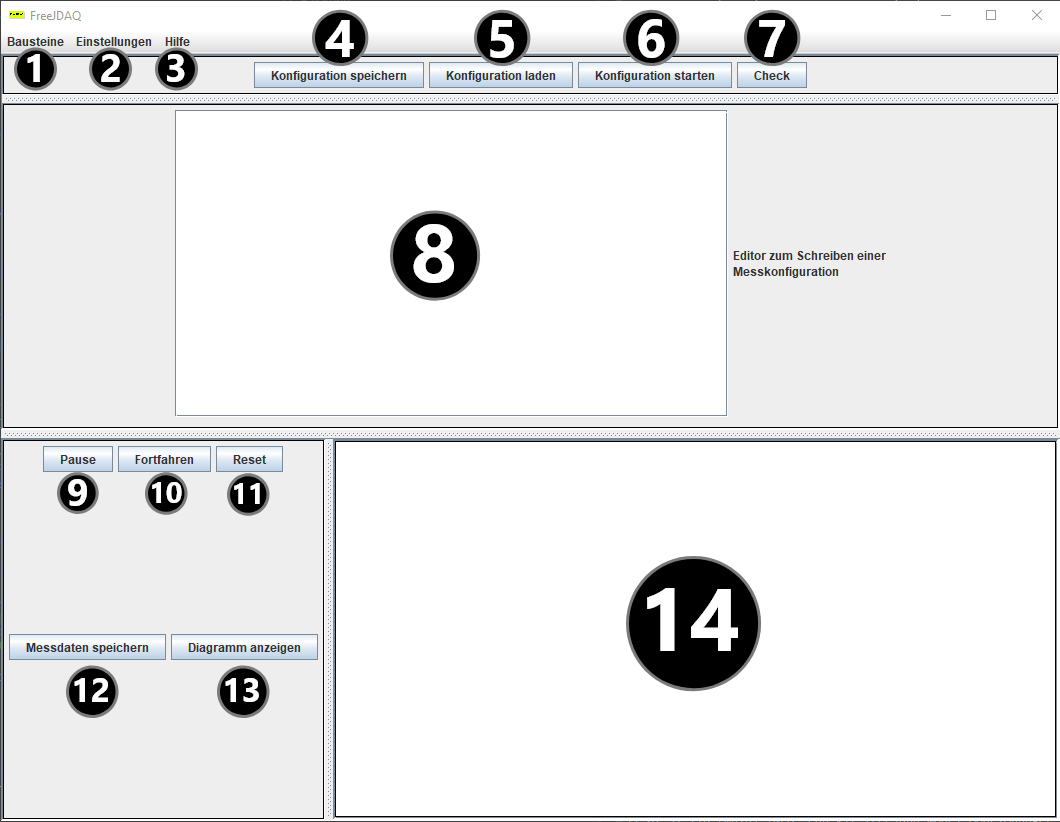
\includegraphics[width = 10cm]{Grafiken/Uebersicht_GUI_Mit_Nummern.png}
        \caption{Die Übersicht über die grafische Benutzeroberfläche von FreeJDAQ. Die Nummern verweißen auf die genauen Beschreibungen, die weiter unten zu finden sind.}
        \label{Uebersicht_GUI_Mit_Nummern}
    \end{center}
\end{figure}

\begin{enumerate}
    \clearpage
    \item
    \begin{flushleft}
        
\includegraphics[width = 1.5cm]{Grafiken/1-Bausteine.png}
    \end{flushleft}

    Öffnet ein Fenster, in dem alle verfügbaren Bausteine angezeigt werden. In diesem Fenster können Bausteineigenschaften bearbeitet werden.
    
    \item
    \begin{flushleft}
        
\includegraphics[width = 2cm]{Grafiken/2-Einstellungen.png}
    \end{flushleft}
    Öffnet ein Fenster, in dem Einstellungen für FreeJDAQ eingesehen werden können. Manche der Einstellungen können angepasst und über den Knopf ''System Einstellungen speichern'' gespeichert werden. Diese beinhalten:
    \begin{itemize}
        \item Fenster-Einstellungen
        \item System-Einstellungen
        \item Messlauf
        \item RasPI
        \item Test Modus
    \end{itemize}
    
    \item
    \begin{flushleft}
        
\includegraphics[width = 1cm]{Grafiken/3-Hilfe.png}
    \end{flushleft}
    
    Öffnet ein Fenster, in dem eine Beschreibung der für das Arbeiten mit FreeJDAQ enthalten ist. Hier können folgende Informationen gefunden werden:
    \begin{itemize}
        \item Systemvorraussetzungen
        \item Softwareanforderungen
        \item Tutorials
    \end{itemize}

    \item
    \begin{flushleft}
        
\includegraphics[width = 3cm]{Grafiken/4-Konfiguration_speichern.png}
    \end{flushleft}
    Öffnet ein Fenster um die aktuelle Konfiguration zu speichern. Der Speicherort und der Name der Konfiguration können, in diesem Fenster, festgelegt werden.
    
    \item
    \begin{flushleft}
        
\includegraphics[width = 3cm]{Grafiken/5-Konfiguration_laden.png}
    \end{flushleft}
    Öffnet ein Fenster zum laden einer Konfiguration.
    
    \item
    \begin{flushleft}
        
\includegraphics[width = 3cm]{Grafiken/6-Konfiguration_starten.png}
    \end{flushleft}
    Startet die aktuell verwendete Konfiguration.
    
    \item
    \begin{flushleft}
        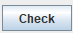
\includegraphics[width = 1.5cm]{Grafiken/7-Check.png}
    \end{flushleft}
    Überprüft die aktuell verwendete Konfiguration auf Lauffähigkeit. Im Fehlerfall wird dem Benutzer eine aussagekräftige Fehlermeldung mitgeteilt.
    
    \item
    %\begin{flushleft}
    %    
\includegraphics[width = 1.5cm]{Grafiken/8-Editor.png}
    %\end{flushleft}
    In diesem Feld können Konfigurationen geschrieben werden. Eine Beschreibung der Sprache, zum schreiben einer Konfiguration, kann in der Hilfe gefunden werden.
    
    \item
    \begin{flushleft}
        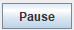
\includegraphics[width = 1.5cm]{Grafiken/9-Pause.png}
    \end{flushleft}
    Pausiert einen Messlauf nachdem er gestartet wurde.
    
    \item
    \begin{flushleft}
        
\includegraphics[width = 2cm]{Grafiken/10-Fortfahren.png}
    \end{flushleft}
    Setzt einen pausierten Messlauf fort.
    
    \item
    \begin{flushleft}
        
\includegraphics[width = 1.5cm]{Grafiken/11-Reset.png}
    \end{flushleft}
    Setzt einen pausierten Messlauf in den Anfangszustand zurück.
    
    \item
    \begin{flushleft}
        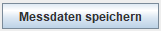
\includegraphics[width = 3cm]{Grafiken/12-Messdaten_speichern.png}
    \end{flushleft}
    Speichert die Daten, die während des Messlaufs bestimmt wurden, am gewünschten Speicherort.
    
    \item
    \begin{flushleft}
        
\includegraphics[width = 3cm]{Grafiken/13-Diagramm_anzeigen.png}
    \end{flushleft}
    Erstellt ein Diagramm aus den Daten, die während des Messlaufs bestimmt wurden.
    
    \item Anzeigefläche für die Messdaten.
    
\end{enumerate}



\section{Beschreibung der Messkonfigurationssprache}


+Im Folgenden Abschnitt wird erklärt, wie man eine Messkonfiguration erstellt und welche syntaktischen Regeln dabei eingehalten werden müssen.  

Eine Messkonfiguration besteht aus 3 zusammenhängenden Teilen., den Bausteinen, den Ein- und Ausgängen der Bausteine und den Verbindungen zwischen Aus- und Eingängen.  

\subsection{Bausteine}

Bausteine bezeichnen einen Knoten für die Datenverarbeitung. Ein Baustein kann 
Sensor, Transformation oder Transformation sein. werden der Messkonfiguration über ihren Namen hinzugefügt. Der Name lässt sich über das Systemmenü „Bausteine“ herausfinden.   
Das Format, in welchem die Bausteine besteht aus der Deklaration für die Bausteine benötigt das Schlüsselwort „blocks:“ Und die Bausteine werden wie folgend deklariert: 

\begin{itemize}

\item[ ] \textbf{blocks: [Baustein1, Baustein2, Baustein3]}

\end{itemize}

\subsection{Ein- und Ausgänge}

Ein- und Ausgänge repräsentieren Schnittstellen für die Verbindung von 2  
Bausteinen. Die Anzahl der Ein- und Ausgänge der Bausteine ist vordefiniert und kann unter „Bausteine -> Bearbeiten“ eingesehen werden. Daher muss die Anzahl der Ein- und Ausgänge in der Messkonfiguration dieser Anzahl entsprechen. Die Namen sind frei wählbar, aber einen eindeutigen und aussagekräftigen vereinfacht das Schreiben der Konfiguration.  
Das Format, in welchem die Ein- und Ausgänge deklariert werden besteht aus dem einem Schlüsselwort und der nachfolgenden Deklaration der Ein- und Ausgänge für jeden Baustein individuell. Das Schlüsselwort ist frei wählbar, jedoch muss die Reihenfolge der Deklaration der Reihenfolge der Baustein-Deklaration entsprechen:  

\begin{itemize}

\item[ ] \textbf{channelListBlock1: [B1out1, B1out2]}
\item[ ] \textbf{channelListBlock2: [T1in, T1out]}
\item[ ] \textbf{channelListBlock3: [R1in1, R1in2]} 

\end{itemize}

\subsection{Verbindungen}

Über Verbindungen zwischen Ein- und Ausgängen der Bausteine wird ein Datenflussmodel erzeugt, über welches die Messdaten laufen.  Eine Verbindung besteht immer zwischen einem Ausgang und einem Eingang, also einem Tupel aus Ausgang und Eingang.   
Das Schlüsselwort für die Verbindungen ist „configuration:“ und die Verbindungen werden wie folgend deklariert:  

\begin{itemize}

\item[ ] \textbf{configuration: [[B1out1, R1in1], [B1out2, T1in], [T1out, R1in2]]}

\end{itemize}

Ein Beispiel für eine solche Konfiguration ist die folgende, welche so in dem Konfigurationsfeld anzeigt werden sollte:

\begin{figure}[htbp]
    \begin{center}
        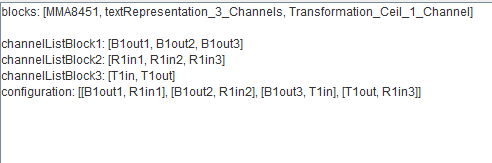
\includegraphics[width = 10cm]{Grafiken/KonfigBsp.png}
        \caption{Beispiel Konfiguration im Konfigurationsfeld}
        \label{KonfigBsp}
    \end{center}
\end{figure}


\clearpage
\section{Umgang mit dem Raspberry Pi}

Folgende Vorbedingungen müssen erfüllt sein:

\begin{itemize}

\item PhyPiDAQ muss auf dem Raspberry Pi installiert sein. (Anleitung)

\item Die gewünschten Sensoren müssen korrekt mit dem Raspberry Pi verbunden sein. Das Vorgehen wird im Handbuch der Sensoren erklärt.

\item Der Raspberry Pi muss so konfiguriert sein, dass eine SSH-Verbindung aufgebaut werden kann, und muss mit dem Endgerät an ein Netzwerk angeschlossen sein.

\end{itemize}

Dann müssen die folgenden Eigenschaften in FreeJDAQ eingestellt werden:

\begin{itemize}

\item IP-Addresse des Raspberry Pi
\item Benutzername und Passwort für die SSH-Verbindung (Standard: \verb:pi: und \verb:raspberry:)
\item Unterordner \textit{examples} des Installationspfads von PhyPiDAQ auf dem Raspberry Pi (z.B. \verb:git/PhyPiDAQ/examples/:)

\end{itemize}

\section{Fehlermeldungen}

Bei Fehlern oder falscher Bedienung der Anwendung werden dem Benutzer Fehlermeldungen angezeigt. Die Fehler unterscheiden sich in 4 Kategorien, welche unten zu sehen sind. Zu jeder Fehlerkategorie gibt es speziellere Fehlerfälle. Diese Fehlerfälle werden in der Fehlerbeschreibung näher beschrieben.

\begin{itemize}


\item[1.] \textbf{Fehler beim Laden einer Konfiguration}: Diese Fehlerkategorie wird gezeigt, wenn es Fehler in der Messkonfiguration gibt.

\item[2.] \textbf{Fehler bei der SSH Verbindung}: Diese Fehlerkategorie wird gezeigt, wenn es zu einem Fehler bei der SSH-Verbindung kommt. Zum Beispiel ist das Passwort oder Benutzername falsch oder es ist keine SSH-Verbindung angelegt.

\item[3.] \textbf{Fehler beim Laden der Bausteine}: Diese Fehlerkategorie wird gezeigt, wenn Bausteine nicht erkannt werden, oder keine ID besitzen.

\item[4.] \textbf{Fehler beim Laden einer Datei}: Diese Fehlerkategorie wird gezeigt, wenn es bei dem Hochladen oder Herunterladen von Dateien von dem Raspberry Pi zu einem Fehler kommt.

\end{itemize}

\section{Limitierung der Anwendung}


\printnoidxglossaries				% generate pdf twice when adding new entries

\end{document}\grid
